\documentclass[tikz,border=14pt]{standalone}
\usetikzlibrary{arrows.meta}
\begin{document}
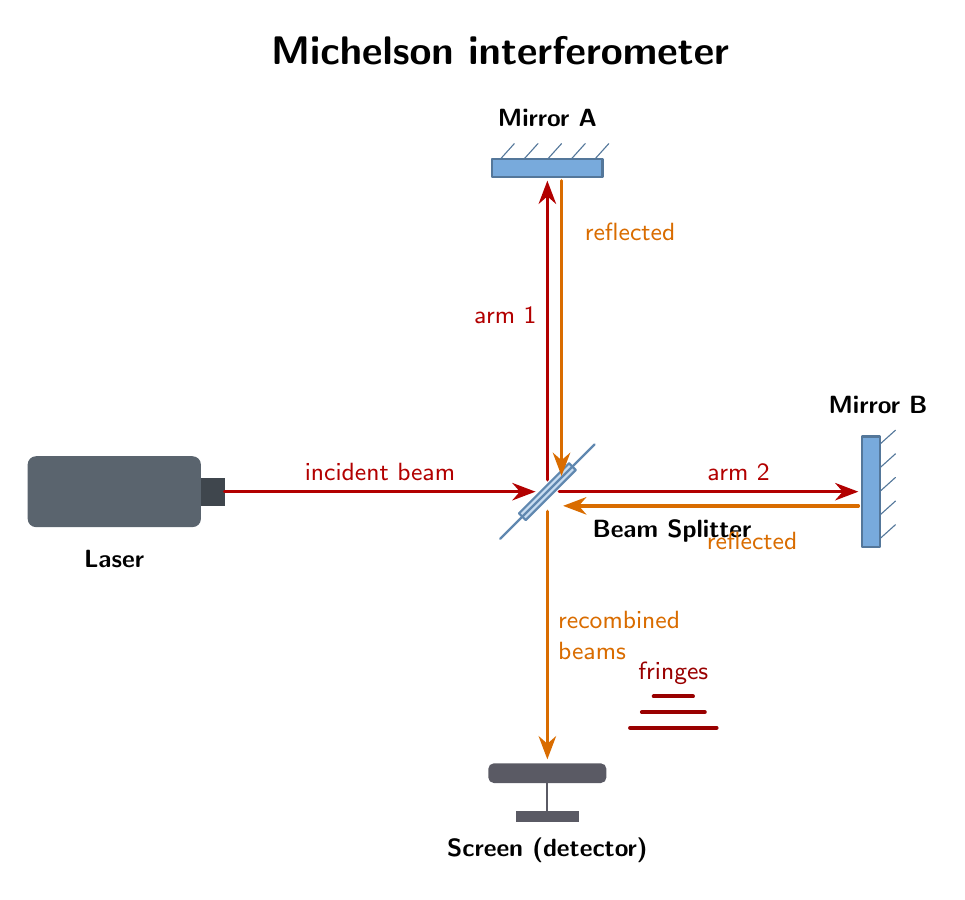
\begin{tikzpicture}[>=Stealth,line cap=round,line join=round,font=\sffamily,
  beam/.style={->,very thick,red!70!black},
  beamr/.style={->,very thick,orange!85!black},
  lab/.style={font=\small\sffamily}]

  \definecolor{laserbody}{RGB}{90,100,110}
  \definecolor{mirrorc}{RGB}{120,170,220}
  \definecolor{screenc}{RGB}{90,90,100}

  % ---- laser (left) ----
  \fill[laserbody,rounded corners=3pt] (-1.6,-0.45) rectangle (0.6,0.45);
  \fill[laserbody!70!black] (0.6,-0.18) rectangle (0.9,0.18);
  \node[lab] at (-0.5,-0.85) {\textbf{Laser}};

  % ---- beam splitter (center, 45 degrees) ----
  \fill[mirrorc!40,draw=mirrorc!80!black,thick,rotate around={45:(5,0)}]
    (4.55,-0.06) rectangle (5.45,0.06);
  \draw[mirrorc!80!black,thick] (4.4,-0.6) -- (5.6,0.6);
  \node[lab,anchor=west] at (5.45,-0.5) {\textbf{Beam Splitter}};

  % ---- mirror A (top, horizontal) ----
  \fill[mirrorc,draw=mirrorc!70!black,thick] (4.3,4.0) rectangle (5.7,4.22);
  \foreach \x in {4.4,4.7,...,5.6} { \draw[mirrorc!70!black] (\x,4.22) -- (\x+0.18,4.42); }
  \node[lab] at (5.0,4.75) {\textbf{Mirror A}};

  % ---- mirror B (right, vertical) ----
  \fill[mirrorc,draw=mirrorc!70!black,thick] (9.0,-0.7) rectangle (9.22,0.7);
  \foreach \y in {-0.6,-0.3,...,0.6} { \draw[mirrorc!70!black] (9.22,\y) -- (9.42,\y+0.18); }
  \node[lab] at (9.2,1.1) {\textbf{Mirror B}};

  % ---- screen (bottom) ----
  \fill[screenc,rounded corners=2pt] (4.25,-3.7) rectangle (5.75,-3.45);
  \draw[screenc,thick] (5.0,-3.7) -- (5.0,-4.1);
  \fill[screenc] (4.6,-4.2) rectangle (5.4,-4.05);
  \node[lab] at (5.0,-4.55) {\textbf{Screen (detector)}};
  % interference fringes drawn beside the screen
  \foreach \y/\w in {-3.0/0.55,-2.8/0.4,-2.6/0.25} {
    \draw[red!60!black,line width=1.4pt] ({6.6-\w},\y) -- ({6.6+\w},\y);
  }
  \node[lab,text=red!60!black] at (6.6,-2.3) {fringes};

  % ---- beams ----
  % incoming
  \draw[beam] (0.9,0) -- (4.85,0) node[lab,midway,above,text=red!70!black] {incident beam};
  % split up to mirror A and back (offset for return)
  \draw[beam] (5.0,0.15) -- (5.0,3.95) node[lab,pos=0.55,left,text=red!70!black] {arm 1};
  \draw[beamr] (5.18,3.95) -- (5.18,0.2);
  % split right to mirror B and back
  \draw[beam] (5.15,0) -- (8.95,0) node[lab,pos=0.6,above,text=red!70!black] {arm 2};
  \draw[beamr] (8.95,-0.18) -- (5.2,-0.18);
  % recombined down to screen
  \draw[beamr] (5.0,-0.25) -- (5.0,-3.4)
    node[lab,midway,right,text=orange!85!black,align=left] {recombined\\beams};

  % small return arrow notes at mirrors
  \node[lab,text=orange!85!black] at (6.05,3.3) {reflected};
  \node[lab,text=orange!85!black] at (7.6,-0.62) {reflected};

  % title
  \node[font=\sffamily\bfseries\Large] at (4.4,5.6) {Michelson interferometer};
\end{tikzpicture}
\end{document}
